\documentclass[11pt,a4paper]{book}
\pagenumbering{arabic} 
\usepackage{titlesec}
\usepackage{setspace}
\usepackage{graphicx}
\usepackage{wrapfig}
\usepackage{color,soul}
\usepackage[customcolors,shade]{hf-tikz}
\usepackage{amsmath}
\usepackage{amssymb}
\usepackage{graphicx}
\usepackage{subfig}
\usepackage{xcolor}
\usepackage{subfig}
\usepackage{sidecap}

\graphicspath{{/Users/giuliodilernia/Documents/Laboratory-Notes/Teoria_Lab2/images/}}

\renewcommand{\baselinestretch}{1.3} 

\titleformat{\chapter}[display]
 {\bfseries\Large}
  {\filright\MakeUppercase{\chaptertitlename} \Huge\thechapter}
  {1ex}
  {\titlerule\vspace{1ex}\filleft}
  [\vspace{1ex}\titlerule]
	
\begin{document}	
\setcounter{chapter}{1}
\chapter{Modelli di probabilit\`{a}}
	
\section{La distribuzione Uniforme}

La distribuzione di probabilit\`{a} uniforme per una variabile aleatoria x continua \`{e} definita come:
\vspace{0.3in}

  \begin{minipage}{.5\textwidth}
    \[ pdf(x) = 
	\begin{cases} 
      \dfrac{1}{b-a} & a \leq x \leq b \\
      0 & altrimenti \\ 
   \end{cases}
\]
  \end{minipage}
  \begin{minipage}{.4\textwidth}
    \centering
    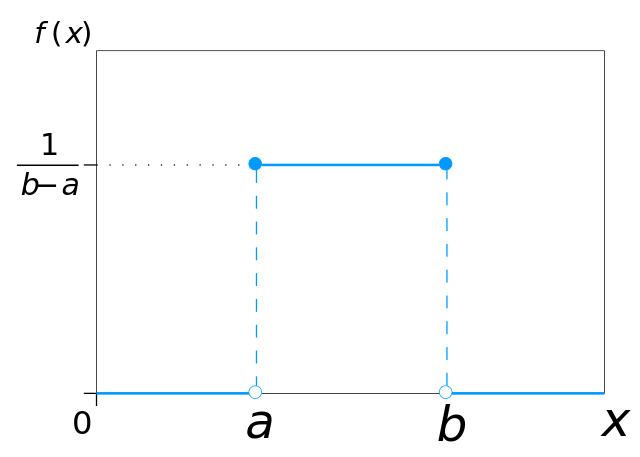
\includegraphics[scale = 0.25]{uniform.png}
 	
  \end{minipage}
\vspace{0.3in}

Tale distribuzione definisce una distribuzione di probabili\`{a} uguale per tutti le variabili aleatorie $x \in \Omega$. 

\subsection{Propriet\`{a} della pdf}
Il valore atteso della distribuzione uniforme e la sua varianza sono date da:

\begin{equation}
	E[x] = \int_{\alpha}^{\beta}{\dfrac{x}{b-a}dx} =\dfrac{b+a}{2} 
\end{equation}

\begin{equation}
	V[x] = \int_{\alpha}^{\beta}{\dfrac{1}{b-a}( x- \dfrac{b+a}{2})^2dx} = \dfrac{(b-a)^2}{12}
\end{equation}
\newline

\noindent Per una distribuzione di questo tipo si ha che la simmetria e la kurtosi rispettivamente hanno valore nullo.\newline
Inoltre tale pdf gode della propriet\`{a} di \textbf{riproduttivit\`{a}} ovvero date due variabili casuali x e y che seguono la pdf uniforme si ha che la nuova variabile aleatoria z = x + y segue una distribuzione di probabilit\`{a} pdf(z) con media $\mu_z = \mu_z + \mu_y$ e varianza $\sigma^2_z = \sigma_x^2 + \sigma_y^2$.\newline

Un'altra propriet\`{a} importante della pdf \`{e} data dal fatto che se si ha una variabile aleatoria x che segue una distribuzione uniforme, la variabile casuale y = f(x) seguir\`{a} anch'essa la medesima distribuzione di probabilit\`{a}.\newline

\noindent Poich\`{e} la pdf possiede una forma analitica \`{e} possibile definirne la cdf:



\vspace{0.3in}

  \begin{minipage}{0.5\textwidth}
  	\begin{equation*}
	cdf(x) = \int_{a}^{x}\dfrac{dx}{b-a} = \dfrac{1}{b-a}(x-a)
\end{equation*}
  \end{minipage}
  \begin{minipage}{.4\textwidth}
    \centering
    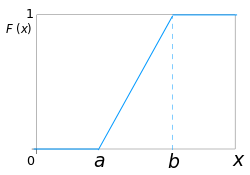
\includegraphics[scale = 0.67]{cdf_uniform.png}

  \end{minipage}
\vspace{0.3in}

\section{La distribuzione Gaussiana (o Normale)}

Data una variabile aleatoria $x \in \Omega $ continua la distribuzione di probabilit\`{a} Gaussiana \`{e} definita come:

\vspace{0.3in}

  \begin{minipage}{0.5\textwidth}
\begin{equation}
	G(x,\mu,\sigma) = \dfrac{1}{\sqrt{2\pi}\sigma} e^{-\dfrac{(x-\mu)^2}{2\sigma^2}}
\end{equation}
  \end{minipage}
  \begin{minipage}{.4\textwidth}
    \centering
    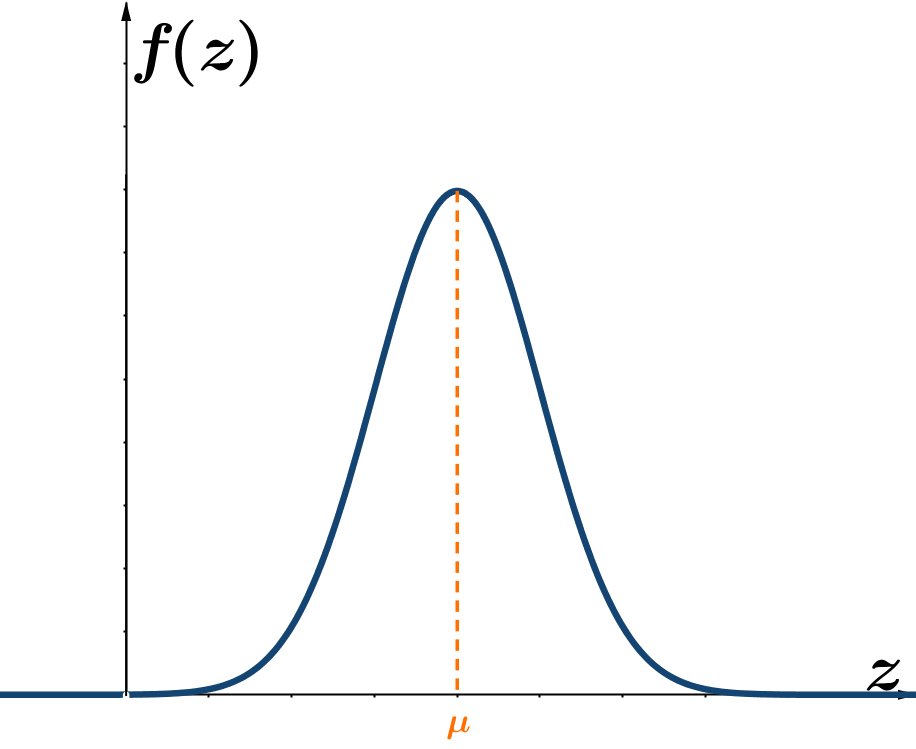
\includegraphics[scale = 0.3]{gaussian.png}

  \end{minipage}
\vspace{0.3in}

Per una distribuzione Gaussiana si ha che la media, la moda e la mediana coincidono essendo una distribuzione simmetrica ovvero $\gamma_{1},\gamma_2 = 0$. Media, Varianza e deviazione standard coincidono con quelle definite al capitolo precedente. Gode della propriet\`{a} di \textbf{riproduttivit\'{a}} definita nella sezione della distribuzione uniforme.\newline

\noindent Una caso speciale di Gaussiana \`{e} quella \textbf{standardizzata} che \`{e} espressa come:

\begin{equation*}
	G(x) = \dfrac{1}{\sqrt{2\pi}}\; e^{-\dfrac{x^2}{2}}
\end{equation*}

\subsection{Distribuzione cumulativa di una Gaussiana}

La pdf Gaussiana non ammette primitiva e la sua cdf viene calcolata numericamente e prende il nome di \textbf{funzione d'errore}, abbreviata con erf(x).

\vspace{0.3in}

  \begin{minipage}{0.5\textwidth}
\begin{equation*}
	erf(x) = \dfrac{1}{\sqrt{2\pi}} \int_{-\infty}^{a}{e^{-\dfrac{x^2}{2}}}
\end{equation*}
  \end{minipage}
  \begin{minipage}{.4\textwidth}
    \centering
    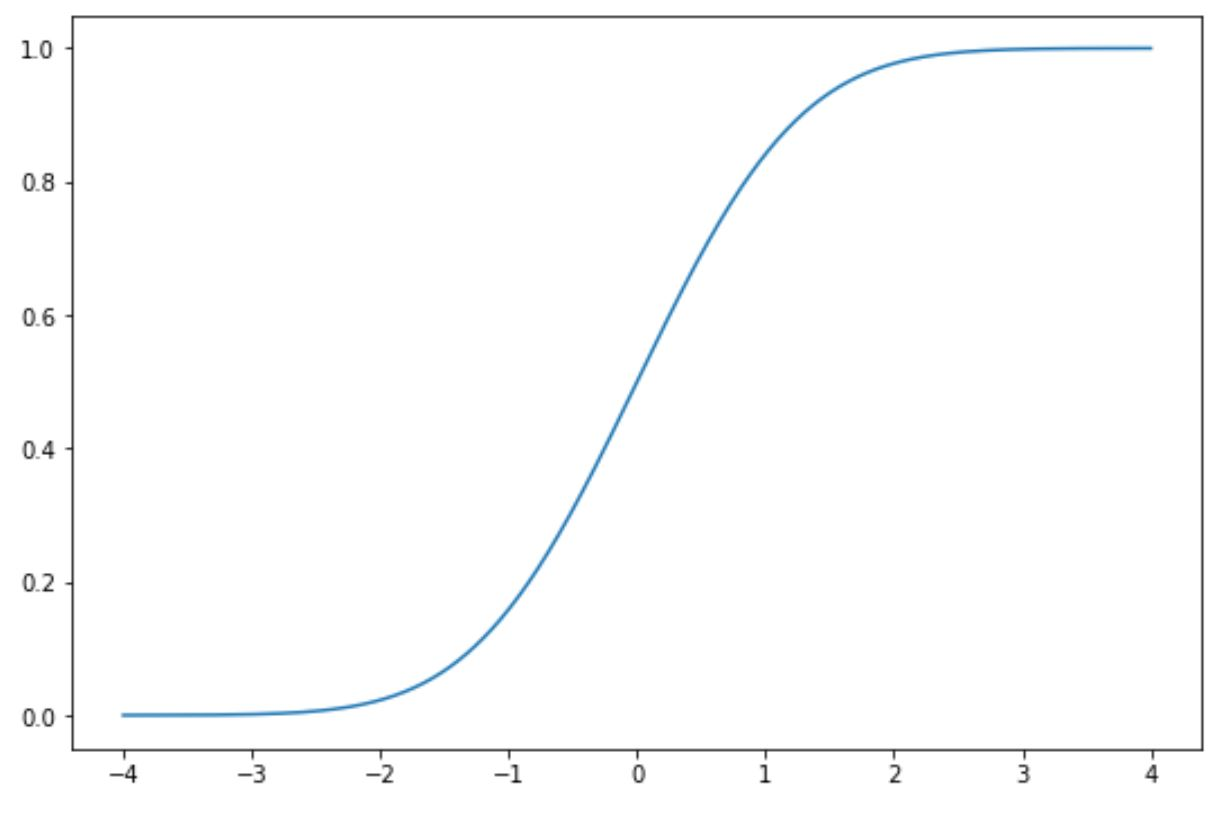
\includegraphics[scale = 0.42]{gauss_cdf.jpeg}

  \end{minipage}
\vspace{0.3in}

\subsection{Teorema Centrale del Limite} 

La distribuzione Gaussiana \`{e} particolarmente importante poich\`{e} per essa vale un importante risultato. 

\subsubsection{Teorema}

Si ipotizzi di avere N variabile aleatorie $\{x_i\}_i^N$ indipendenti tra loro e ciascuna di esse segue una distribuzione di probabilit\`{a} $f_i(x)$ con $E[x_i] < \infty$ e $V[x_i] < \infty$, e definiamo una nuova variabile aleatoria $s = \sum_{i=1}^Nx_{i}$ che segue una distribuzione pdf(s), allora si avr\`{a} che al crescere del numero di variabili:
\begin{equation*}
	\lim_{N \rightarrow \infty} pdf(s) \rightarrow G(s,\mu_s,\sigma_s)
\end{equation*}

dove $\mu_s =\sum_{i=1}^N \mu_i$ e $\sigma_s^2 = \sum_{i=1}^N \sigma^2_i$ .

\subsubsection{Corollario della media}

Date N variabili aleatorie $\{x_{i}\}_{i}^N$ indipendenti ed identicamente distribuite, ovvero che per ogni variabile si ha la stessa distribuzione di probabilit\`{a} f(x) e ipotizzando che $\forall i$ si ha che $\mu_i$ e $\sigma_i^2$ siano finite , definita una nuova variabile aleatoria $\overline{x} = \dfrac{\sum_{i=1}^N x_{i}}{N}$ che segue una pdf $f(\overline{x})$, si ha che al crescere del numero di variabili:

\begin{equation*}
	\lim_{N \rightarrow \infty} f(\overline{x}) \rightarrow G(\overline{x},\mu,\frac{\sigma}{\sqrt{N}})
\end{equation*}

dunque si ha che la pdf delle medie campionarie di un campione che cresce converge alla distribuzione Gaussiana.


\subsubsection{Conseguenze del TCL}

 Quando effettuiamo una misura in un esperimento in generale possiamo definirla come la somma del valore vero $x_0$ e di un errore $\epsilon$ che \`{e} una variabile aleatoria.
 
 \begin{equation*}
 	x = x_0 + \epsilon
 \end{equation*}

la misura cos\`{i} ottenuta segue una pdf(x), il che equivale a dire che segue la pdf($\epsilon$). Ipotizziamo di effettuare pi\`{u} misure di una stessa variabile aleatoria e di volerne calcolare la media, in realt\`{a} la media che calcoliamo \`{e} quella degli errori $\epsilon$, assummendo che $V[\epsilon_i] < \infty$ e $E[\epsilon_i] < \infty$ e che le $\{\epsilon_i\}_{i}^N$ siano indipendenti tra loro, possiamo applicare il TCL e dunque la  pdf($\overline{\epsilon}$) $\rightarrow$ G($\overline{\epsilon}$,$\mu$,$\frac{\sigma}{\sqrt{N}}$). Quindi l'errore medio delle misurazioni di un esperimento segue una distribuzione di probabilit\`{a} Gaussiana.

\section{Distribuzione di probabilit\`{a} Log-normale}

Presa una variabile aleatoria $x \in \Omega $ che segue una distribuzione Gaussiana, costruiamo una nuova variabile aleatoria y legata alla precedente dalla relazione $y = e^x$, in questo modo si definisce la distribuzione log-normale applicando un cambio di variabile alla G(x) di partenza, il metodo con cui si effettua un cambio di variabile verr\`{a} presentato nei capitoli successivi.

\begin{equation*}
	f(x,\mu,\sigma) = \dfrac{1}{\sqrt{2\pi}\sigma}\;\dfrac{1}{x}\; e^{-\frac{(log(x)-\mu)^2}{2\sigma^2}}
\end{equation*} 

\subsection{Propriet\`{a} della log-normale}

Il valore di aspettazione e varianza della log-normale sono dati da:

\begin{equation}
	E[x] = e^{(\mu + \frac{1}{2}\sigma^2)}
\end{equation}

\begin{equation}
	V[x] = e^{(2\mu + \sigma^2)}e^{(\sigma^2-1)}
\end{equation}

\section{Distribuzione di Probabilit\`{a} di Bernoulli}

Sia $x \in \Omega = \{0,1\}$ una variabile aleatoria discreta, a cui \`{e} possibile associare una probabilit\`{a} $p \in [0,1]$. Definiremo che l'evento x si \`{e} realizzato con successo quando P(x = 1) = p, mentre l'insuccesso con P(x = 0)= (1-p). Dunqua la pdf(x) \`{e} data da:

\begin{equation*}
	f(x,p) = p^x(1-p)^{1-x}
\end{equation*}

\subsection{Propriet\`{a} della distribuzione Bernoulliana}

Per una distribuzione di Bernoulli media e varianza sono date:

\begin{equation}
	E[x] = \sum_{\{0,1\}}xf(x,p) = p
\end{equation}

\begin{equation}
	V[x] = \sum_{\{0,1\}}(x-p)^2f(x,p) = p(1-p)
\end{equation}

\section{Distribuzione di Probabilit\`{a} Binomiale}

Si consideri un insieme di N osservazioni indipendenti, che seguono una distribuzione di Bernoulli. Contiamo il numero di volte k in cui l'evento ha successo rispetto al numero di tentativi effettuati, tale insieme \`{e} il nostro campione. Se si ripete l'esperimento effettuando sempre N tentativi, il numero di successi n sar\`{a} distribuita secondo la distribuzione binomiale:

\begin{equation*}
	B(k \vert N,p) = \binom{N}{k}p^k(1-p)^{N-k}
\end{equation*} 
\newline
notare che a differenza delle distribuzioni viste fino ad ora, la distribuzione binomiale in realt\`{a} rappresenta la probabilit\`{a} stessa di una variabile aleatoria k, come anche la Bernoulliana.

\subsection{Propriet\`{a} della distribuzione binomiale}

Per una distribuzione binomiale il valore di aspettazione e la varianza sono definite da :

\begin{equation}
	E[k] = \sum_{k}^\infty k \binom{N}{k}p^k(1-p)^{N-k} = Np
\end{equation}

\begin{equation}
	V[k] = E[k^2] - E[k]^2 = Np(1-p)
\end{equation}

\noindent la simmetria \`{e} data da:
\begin{equation}
	\gamma_1 = \dfrac{1-2p}{\sqrt{Np(1-p)}}
\end{equation}

dove $\gamma_1 \rightarrow 0 $ per $N \rightarrow \infty $ o per $p = \frac{1}{2}$.\newline

la kurtosi invece si esprime come:
\begin{equation}
	\gamma_2 = \dfrac{1-6p}{Np(1-p)}
\end{equation}

dove $\gamma_2 \rightarrow 0$ per $N \rightarrow \infty$ e $p = \frac{1}{6}$.
Inoltre la distribuzione binomiale gode della propriet\`{a} di \textbf{riproduttivit\`{a}}
\subsection{La densit\`{a} di probabilit\'{a} di un'istogramma}



Consideriamo di avere una variabile aleatoria x di cui effettuiamo N misurazioni, ciascuna misurazione segue una pdf(x). 

\begin{wrapfigure}{l}{0.\textwidth}
\centering

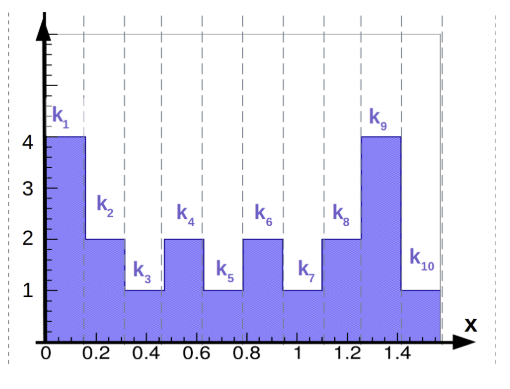
\includegraphics[scale = 0.33]{binning}	

\end{wrapfigure}

\noindent L'operazione \`{e} equivalente a campionare N volte una pdf(x). Posto che le $\{x_{i}\}_{i}^N$ misure siano il campione di riferimento, la statistica si pone obbiettivo quello di ricostruire partendo dal campione le caratteristiche di una pdf(x).
\begin{wrapfigure}{r}{0.\textwidth}
\centering
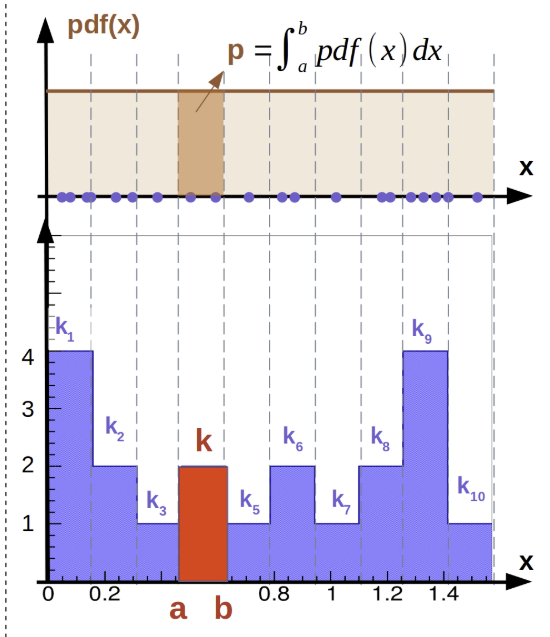
\includegraphics[width = 1.9in]{Bernouli_Histo}	

\end{wrapfigure}
\noindent Per farlo si procede a costruire un istogramma e a contare il numero di eventi $k_{i}$ che cadono all'interno di un bin e rappresentare tale numero con una barra. Il numero di misure $k_i$ che cade all'intero di un bin \`{e} una variabile aleatoria.


Di conseguenza studiando il comportamento di un singolo bin [a,b), il numero di misure $k_{i}$ \`{e} descritto da una distribuzione di probabilit\`{a}, poich\`{e} un fenomeno cade o non cade all'interno dell'intervallo la pdf($k_i$) \`{e} quella di Bernoulli. 

Reiterando l'esperimento sullo stesso bin il numero di successi $k_{i}$ seguir\`{a} una pdf(k) di una binomiale $B(k \vert N,p)$ dove la probabilit\`{a} \`{e} $ p = \int_{a}^{b}{pdf(x)dx}$ sull'intervallo del bin associato.

 Un conteggio di misure \`{e} soggetto a fluttuazioni statistiche, e al crescere del numero delle misure l'istogramma assumer\`{a} la distribuzione di probabilit\`{a} pdf(x) della variabile aleatoria X misurata.
\newline
\noindent Se ipotizziamo che X abbia una distribuzione uniforme, valore di aspettazione e varianza di un conteggio coincideranno con quella della distribuzione Binomiale.

I metodi statisti che possono essere applicati a misure binnate richiedono che i conteggi $k_{i}$ siano variabili aleatorie indipendenti, affinch\`{e} tale condizione risulti essere verificata si hanno due strategie possibili:

\begin{itemize}
\item
\noindent Se la dimensione dei bin \`{e} piccola e la probabilit\`{a} \`{e} sufficientemente piccola allora la covarianza \`{e} pressoch\`{e} nulla. Di conseguenza le variabili $k_i$ sono indipendenti tra loro e dunque ciascuan distribuita come una binomiale.
\item
\noindent Se il numero di eventi N \`{e} molto grande e la probabilit\`{a} $p_i$ \`{e} piccola la distribuzione di probabilit\`{a} dei conteggi \`{e} approssimabile a quella di una distribuzione Poissoniana. 
\section{Distribuzione Multinomiale}

\end{itemize}

Considerando quando discusso nella sezione precedente per ogni singolo bin che si \`{e} costruito nell'istogramma, si definisce una probabilit\`{a} multinomiale:

\begin{equation}
	Multi(k_1,k_2,...,p_1,p_2,...) = \dfrac{N!}{k_1!\cdot k_2! \cdots}p^{k_{1}}p^{k_2}\cdots
\end{equation}
\newline
\noindent Valore di aspettazione e varianza rimangono le medesime per ogni singolo bin, solo che i conteggi $k_i$ non sono variabili aleatorie indipendenti tra loro, in questo caso si ha la \textbf{covarianza}:

\begin{equation}
	cov[k_i,k_j] = -N \cdot p_i \cdot p_j 
\end{equation}

\section{Distribuzione di Poisson}

La distribuzione di Poisson \`{e} una distribuzione di probabilit\`{a} discreta che esprime la probabilit\`{a} che un numero di eventi indipendenti si verifichi in un certo intervallo di spazio o tempo fissato con una frequenza media costante. il verificarsi dell'evento a un tempo t non influenza il verificarsi del medesimo in un intervallo di tempo successivo o precedente  al tempo t.
La probabilit\`{a} di contare k eventi in un intervallo di tempo unitario \`{e}:

\begin{equation}
	Poiss(k,\lambda) = \dfrac{e^{-\lambda} \cdot \lambda^k}{k!}
\end{equation}

lo spazio campione rispetto alla quale \`{e} definita \`{e} tutto $\mathbb{N}$



\subsection{Propriet\`{a} della distribuzione di Poisson}

Il valore di aspettazione e la varianza della distribuzione di Poisson sono:

\begin{equation}
	E[k] = \sum_{k=0}^{\infty}k \cdot \dfrac{e^{-\lambda} \cdot \lambda^k}{k!} = \lambda 
\end{equation}

\begin{equation}
	V[k] = \sum_{k=0}^{\infty} (k - \lambda)^2 \cdot \dfrac{e^{-\lambda} \cdot \lambda^k}{k!} = \lambda 
\end{equation}

si nota che all'aumentare della media aumenta anche la varianza. \newline

L'indice di simmetria e kurtosi sono dati da:

\begin{equation}
	\gamma_1 = \dfrac{1}{\sqrt{\lambda}}
\end{equation}

\begin{equation}
	\gamma_2 = \frac{1}{\lambda}
\end{equation}

per $\lambda \rightarrow \infty $ la distribuzione di Poisson diventa pi\`{u} simmetrica. Inoltre la distribuzione di Poisson gode della propriet\`{a} di \textbf{riproduttivit\`{a}}.


\subsection{Da eventi Poissoniani all'esponenziale}

Il modello su cui si basa la distribuzione di Poisson \`{e} dato dalle seguenti assunzioni:

\begin{itemize}
	\item la probabilit\`{a} che un evento avvenga in un intervallo di tempo [t,t+dt] \`{e} data da $p\cdot dt$, dove p \`{e} un valore costante e indipendente da t;
	\item la probabilit\`{a} di avere pi\`{u} di un evento nell'intervallo dt \`{e} nulla.
	\item gli eventi sono indipendenti tra loro.
\end{itemize}

Definiamo E = \{ nessun evento avvenuto in [0,t+dt]\} e la funzione q(t) = \{probabilit\`{a} di nessun evento in [0,t]\}, posta I come l'informazione a priori (ex: tempo di decadimento medio) si ha che la probabilit\`{a} che si verifichi E essendosi gi\`{a} verificato I \`{e}:

\begin{equation}
	P(E\vert I) \equiv q(t+dt)
\end{equation} 

Dove q ha come argomento la lunghezza degli intervalli di tempo; possiamo riformulare E come l'intersezione di due eventi $E_1 =$ \{0 eventi in [0,t] \} ed $E_2 = $ \{ 0 eventi in [t,t+dt]\}, dunque 2.19 pu\`{o} essere riscritta come:

\begin{equation*}
	P(E \vert I) = P(E_1,E_2 \vert I) = P(E_1 \vert I)P(E_2 \vert E_1 ,I)
\end{equation*}

poich\`{e} per ipotesi $E_{1}$ ed $E_{2}$ sono indipendenti dato che il verificarsi di un evento in un intervallo di tempo non influenza il verificarsi del medesimo evento in un intervallo successivo si ha che:

\begin{equation}
	P(E \vert I) = P(E_1 \vert I)P(E_2 \vert I)
\end{equation}

dove $P(E \vert I) = q(t+dt)$ , $P(E_1 \vert I) = q(t)$ e $P(E_2 \vert I) = 1-pdt$. Dunque:

\begin{equation}
	q(t+dt) = q(t)\cdot (1-pdt) \Rightarrow \dfrac{q(t+dt)-q(t)}{dt} = -q(t)p
\end{equation}

questo \`{e} equivalente all'equazione differenziale al primo ordine:

\begin{equation*}
	\dfrac{dq}{q} = -p \cdot dt \iff q(t) = q(0)e^{-pt}
\end{equation*}

dove q(0) \`{e} determinata normalizzando la distribuzione di probabilit\`{a}. \textcolor{cyan}{Per eventi che occorono in modo Poissoniano la probabilit\`{a} di non avere eventi in un intervallo [0,x] \`{e} data da una esponenziale}.

Per comodit\`{a} poniamo q(0)=1. Definiamo $A = \{ 1 \; evento \; in \; [t_1,t_1+dt_1] \}$ ed B = \{ 0 eventi in [0,$t_1$]\} definiamo:

\begin{equation}
	P(A,B \vert I) = P(A \vert I) \cdot P(B \vert I) = e^{-pt}(p \cdot dt)
\end{equation} 

ipotizzando di costruire una catena di eventi in cui si realizza e non si realizza un evento per tempi ordinati si ha che:
\begin{equation}
	P(A,B \vert I) = e^{-pt_1} \cdot p \cdot dt_1 \cdot e^{-p(t_2-t_1)} \cdot p \cdot dt_2 \cdots = e^{-pt}p^ndt_1 \cdots dt_n
\end{equation}

Per definire una probabilit\`{a} che si realizzino n eventi in un intervallo di tempo [0,t], a prescindere dal tempo preciso in cui avvengono, dobbiamo sommare le probabilit\`{a} definite in (2.23):

\begin{equation}
	P(n \vert p,t,I) = e^{-pt}p^n \int_0^{t_2}dt_{1} \cdot \int_{0}^{t^3}dt_{2} \cdots \int_{0}^{t}dt_n
\end{equation}

il prodotto d'integrali ha come soluzione $\frac{t^n}{n!}$ e dunque:

\begin{equation}
	P(n \vert p,t,I) = \dfrac{(pt)^n}{n!}e^{-pt} = \dfrac{\lambda^n}{n!}e^{-\lambda}
\end{equation} 

\section{Distribuzione Esponenziale}

La distribuzione esponenziale \`{e} la distribuzione dei tempi che intercorrono tra due eventi Poissoniani, ovvero la probabilit\`{a} che nessun evento si verifichi. Infatti consideriamo k il numero di eventi definiti da una pdf Poissoniana con frequenza p, avvenuti in un intervallo di tempo [0,t]. Allora si ha:

\begin{equation*}
	P(k,p) = \dfrac{(pt)^k}{k!}e^{-pt}
\end{equation*}
\newline
 Se misuriamo la probalit\`{a} che nessun evento si verifichi in un tempo $t < T$ si avr\`{a}:

\begin{equation*}
	P(0 \vert p,t) = \dfrac{(pt)^0}{0!}e^{-pt} = e^{-pt}
\end{equation*}
\newline
 e si ha dunque una pdf Poissoniana. Se rileviamo il medesimo evento per $T > t$ si avr\`{a} che la probabilit\`{a} dell'evento avvenuto al tempo T \`{e} descritta dalla medesima pdf per il tempo t antecedente:

\begin{equation*}
	P(0 \vert p, T>t) = P(0 \vert p, t) = e^{-pt}
\end{equation*}
 Dunque la distribuzione di probabilit\`{a} che intercorre da tra due eventi Poissoniani \`{e} esponenziale.
\begin{figure}[ht]
\vspace{0.2in}
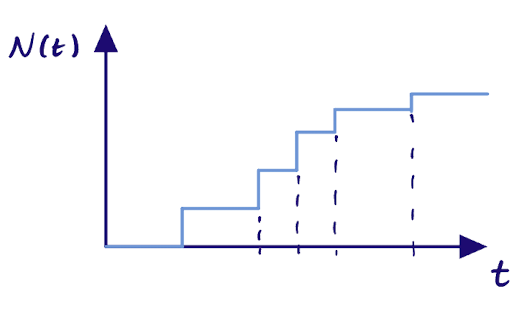
\includegraphics[scale = 0.45]{pois}	
\centering
\vspace{0.2in}
\end{figure}

ed \`{e} definita da:

\begin{equation}
	pdf(t,\lambda) = \lambda \cdot e^{-\lambda t}
\end{equation}

dove $\tau$ = E[t] \`{e} il tempo medio tra due eventi consecutivi, e vale la relazione $\lambda = \frac{1}{\tau}$ dove $\lambda$ \`{e} il parametro della Poissoniana che determina la frequenza media di eventi. 

\subsection{Propriet\'{a} della distribuzione esponenziale}

Il valore di aspettazione e varianza sono date dalle quantit\`{a}:

\begin{equation}
	E[t] = \tau = \dfrac{1}{\lambda}
\end{equation}

\begin{equation}
	V[t] = \tau^2 = \dfrac{1}{\lambda^2}
\end{equation}

mentre i parametri di simmetria della distribuzione dati da simmetria e kurtosi:

\begin{equation}
	\gamma_1 = 2
\end{equation}

\begin{equation}
	\gamma_2 = 6
\end{equation}

come si osserva dai momenti essendo $\gamma_1$ e $\gamma_2$ costanti la distribuzione esponenziale non pu\`{o} tendere ad una Gaussiana al crescere del numero die venti.

\subsection{Decadimento Radioattivo}

Si consideri un campione di materiale radioattivo contenente $N_{0}$ nuclei al tempo t=0 per un singolo nucleo padre la probabilit\`{a} di decadimento segue una distribuzione esponenziale il cui $\tau$ tempo medio di decadimento \`{e} dato dalla meccanica quantistica. Gli eventi di decadimento sono \textbf{indipendenti} tra di loro.
\newline
La variazione del numero dei nuclei in un intervallo di tempo $\Delta t$ sar\`{a} proporzionale al numero di nuclei restanti:

\begin{equation}
	-\dfrac{dN}{dt} = \lambda N
\end{equation}

dove $\lambda$ \`{e} la frequenza media di decadimento. Di conseguenza il decadimento radioattivo \`{e} definito dalla funzione:

\begin{equation}
	N(t) = N_{0}e^{-\lambda t}
\end{equation}

che possiamo riscrivere come :

\begin{equation}
	N(t) = N_{0} e^{-\frac{t}{\tau}}
\end{equation}

Se $\tau >> t$ tempo di osservazione, la frequenza media dei decadimenti \`{e} costante nel tempo e di conseguenza la probabilit\`{a} di osservare k decadimenti in un campione di N nuclei \`{e} data dalla distribuzione di Poisson con $\lambda = \frac{1}{\tau}$.

\section{Comportamenti Asintotici delle distribuzioni}

\subsection{Propriet\`{a} asintotiche della Binomiale e Poissoniana}

\subsubsection{Binom(k$\vert$N,p) $\rightarrow$ Poisson(k,$\mu = N \cdot p$)}
La relazione tra distribuzione Binomiale e Poissoniana si costruisce assumendo di prendere un intervallo $\Delta t$ e di dividerlo in N intervalli di dimensione dt tali per cui:

\begin{itemize}
	\item in ciascun dt cada uno solo evento( tale ipotesi \`{e} verificata solo se il numeri di eventi \`{e} molto grande);
	\item la probabilit\`{a} in un singolo intervallo dt \`{e} $p = \dfrac{\lambda}{N}$ ed \`{e} finita;
	\item gli eventi che cadono in ogni intervallo dt sono indipendenti tra loro.
	
\end{itemize}

Essendo gli eventi indipendenti tra loro per ipotesi ciascuno di essi segue una distribuzione di Bernoulli. Tali condizioni consentono di usare una distribuzione binomiale per descrivere eventi Poissoniani.

Per induzione si ha che per k=0 posto $\lambda = N \cdot p$

\begin{equation*}
	B \Big (0\vert N, \dfrac{\lambda}{N} \Big ) = \Big (1- \dfrac{\lambda}{N} \Big )^N =_{N \rightarrow \infty} \dfrac{\lambda^0}{0!}e^{-\lambda}
\end{equation*}

dunque la relazione per k-1 sar\`{a} verificata e:

\begin{equation*}
	B \Big (k-1\vert N,\frac{\lambda}{N} \Big ) =_{N \rightarrow \infty} \dfrac{\lambda^{k-1}}{(k-1)!} e^{- \lambda}
\end{equation*}

Allora si dimostra che dall'espressione binomiale:

\begin{equation*}
	\dfrac{B \Big (k  \vert N , \dfrac{\lambda}{N}\Big)}{B \Big(k-1 \vert N, \dfrac{\lambda}{N} \Big) } = \dfrac{Np- (k-1)p}{k(1-p)} \approx_{p \rightarrow 0} \dfrac{\lambda}{k}
\end{equation*}


 dunque:
 
 \begin{equation*}
 	B \Big (k  \vert N , \dfrac{\lambda}{N}\Big) = \dfrac{\lambda}{k} \cdot B \Big(k-1 \vert N, \dfrac{\lambda}{N} \Big) \rightarrow \dfrac{\lambda^{k}}{k!} e^{-\lambda}
 \end{equation*}
\newline

Si dimostra inoltre che data una distribuzione Binomiale $B(k \vert N,p) \rightarrow G(k,\mu,\sqrt{\mu})$ al crescere del numero di misure $N \rightarrow \infty $ per $\mu = N \cdot p$ costante.
\newline

Vale anche il fatto che per una Poissoniana si ha $Poiss(k,\lambda) \rightarrow G(k,\lambda, \sqrt{\lambda})$ per $\lambda \rightarrow \infty $.

 
\begin{figure}[!ht]
\vspace{0.2in}
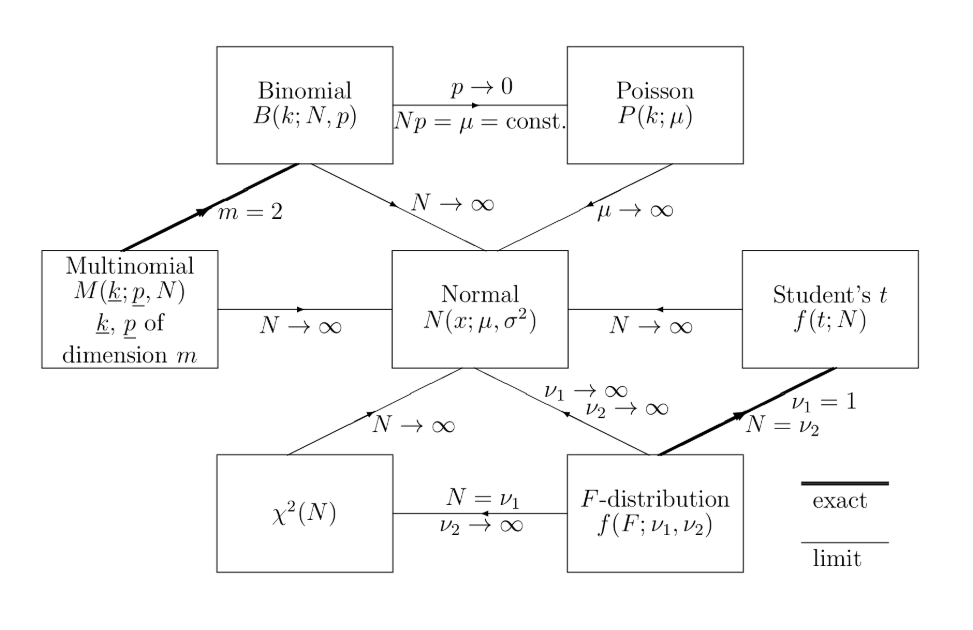
\includegraphics[scale = 0.4]{Asymptotic_map}	
\centering
\vspace{0.2in}
\caption{Mappa delle distribuzioni asintotiche}
\end{figure}


\section{Distribuzione di $\chi^2$}


La distribuzione di $\chi^2$ nasce nel contesto della modellazione di dati per la stima di parametri usando i metodi di maximum likelihood e minimi quadrati. Dato un campione di n punti $\{(x_i,y_i)\}_{i}^N$ e un modello $f(x, \bold{\underline{\theta}})$, dipendente da m parametri $\underline{\theta}$ si valuta la bont\`{a} del modello nell'approssimare i dati usando la funzione di $Q^2$ definita come:

\begin{equation}
	\chi^2 = \sum_{i=1}^{n}\dfrac{[y_i - f(x_i,\underline{\theta})]}{\sigma^2_i}
\end{equation}

dove le $\sigma^2_i$ sono gli errori sulle n misure di $y_i$. 
\newline
Per le misure y che seguono una pdf Gaussiana, la pdf del $\chi^2$ \`{e} data distribuzione:


\vspace{0.3in}

  \begin{minipage}{0.5\textwidth}
\begin{equation*}
	\chi^2 = \dfrac{1}{2^{\frac{n}{2}}\Gamma(\frac{n}{2})}z^{(\frac{n}{2}-1)}e^{-\frac{z}{2}}
\end{equation*}
  \end{minipage}
  \begin{minipage}{.4\textwidth}
    \centering
    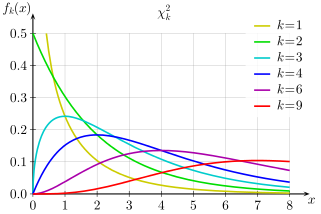
\includegraphics[scale = 0.545]{chi2.png}

  \end{minipage}
\vspace{0.3in}

dove \textbf{n} prende il nome di \textbf{numero di gradi di libert\`{a}} e $\Gamma(x)$ \`{e} la funzione gamma.

\begin{wrapfigure}[7]{l}{0.\textwidth}
\centering

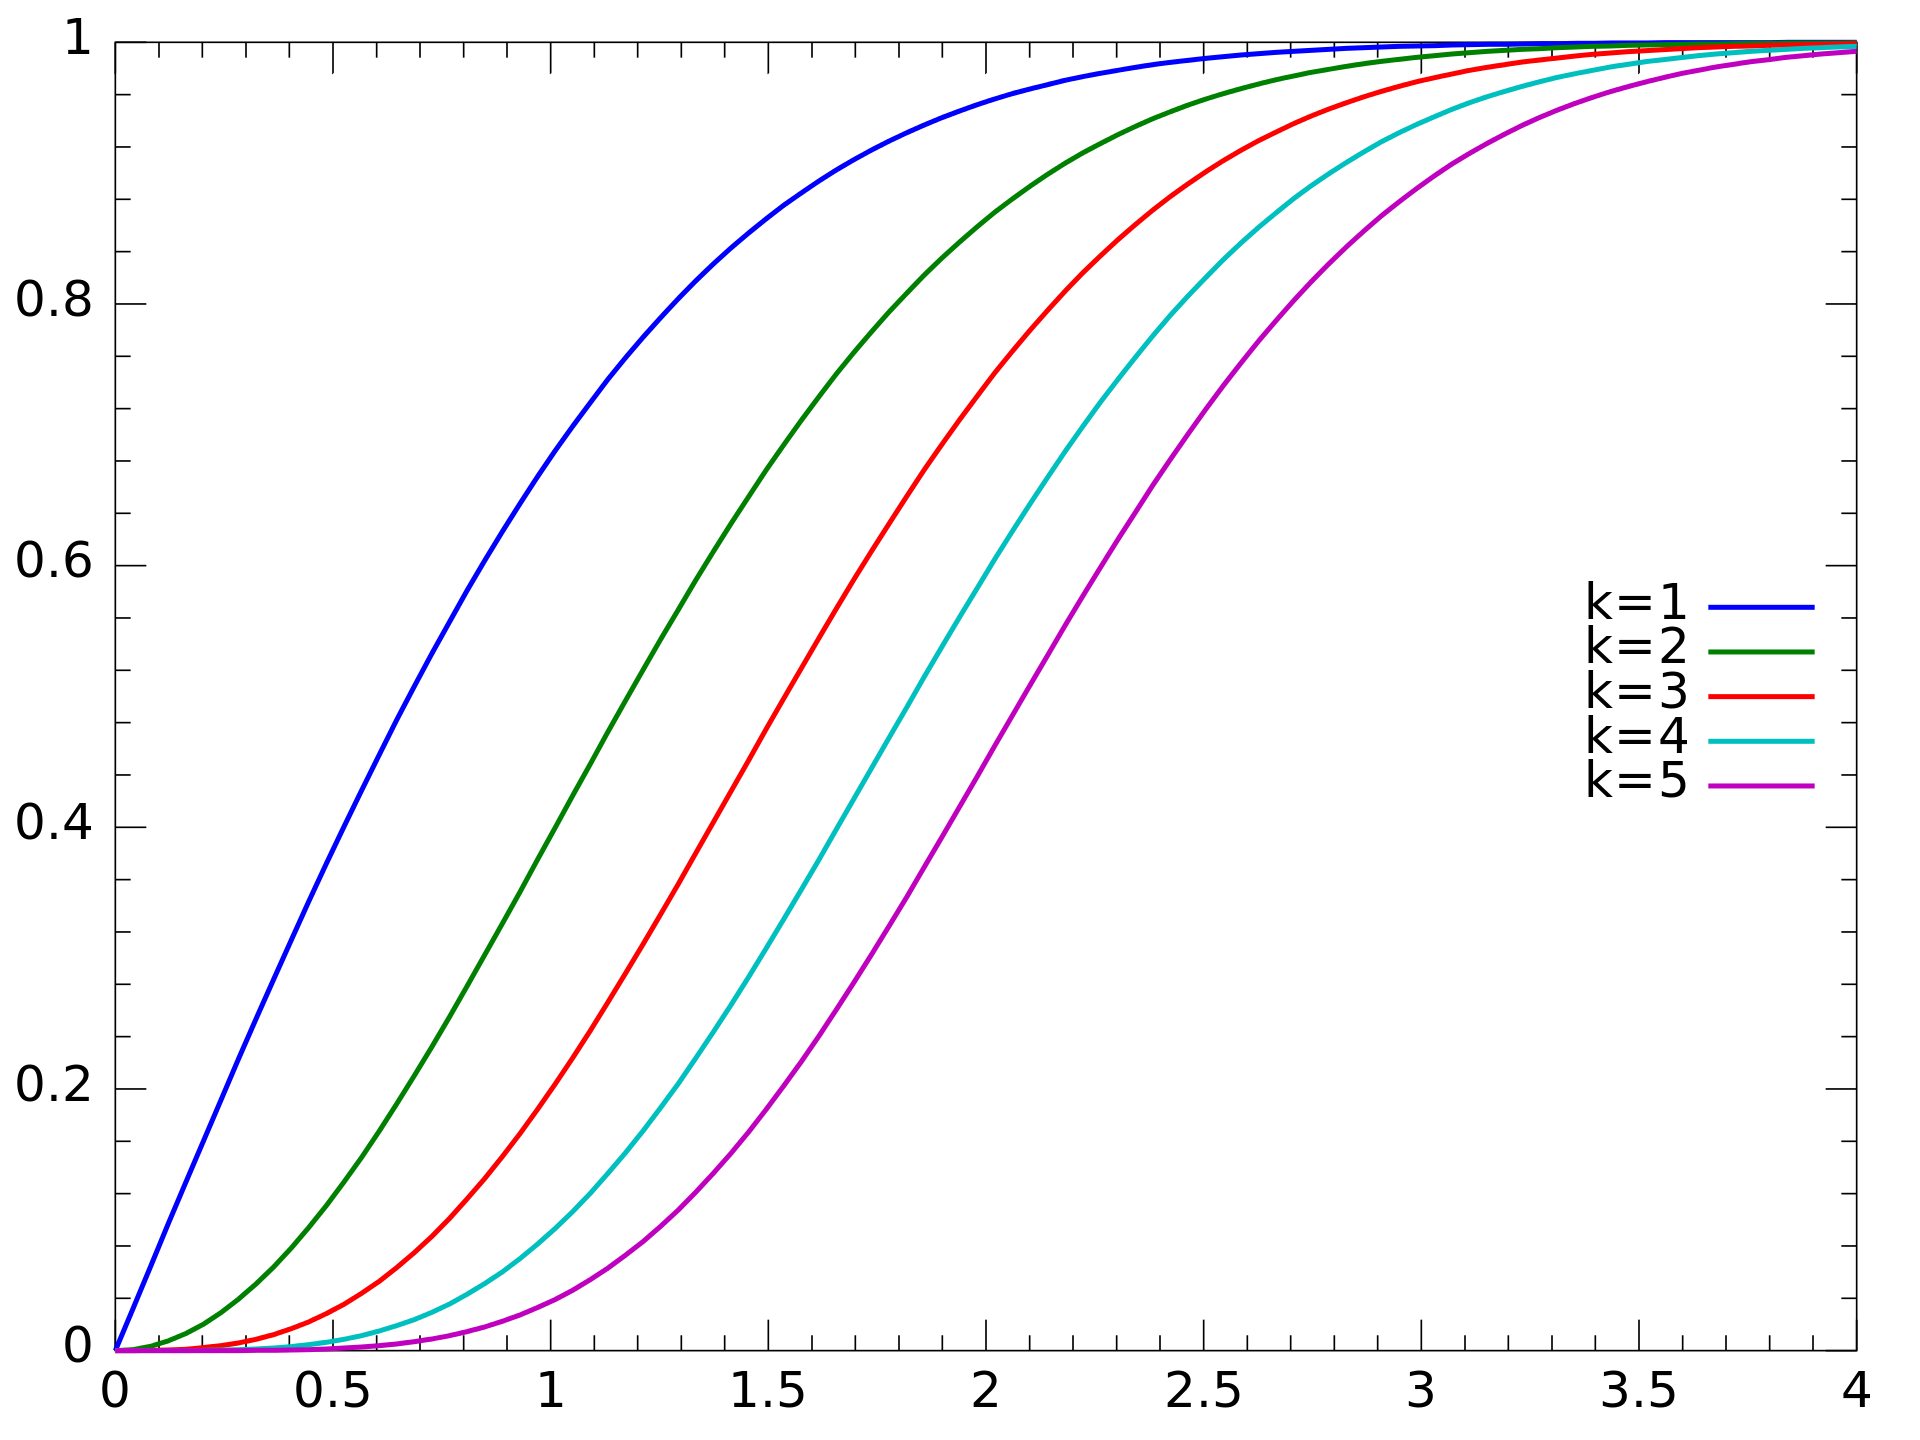
\includegraphics[scale = 0.1]{chiCdf.png}	

\end{wrapfigure}

\noindent La distribuzione di $\chi^2$ possiede una distribuzione cumulativa e gode delle seguenti propriet\`{a}:

\begin{itemize}
	\item \textbf{media:} E[n] = n
	\item \textbf{Varianza:} V[n] = 2n
	\item \`{e} riproduttiva
	\item \textbf{moda:} n-2
	\end{itemize}
	
\subsubsection{$\chi^2$ ridotto}

Si definisce $\chi^2$ ridotto data dal rapporto $\frac{\chi^2_N}{n}$ e la sua media \`{e} pari a 1.

 
\begin{figure}[ht]
\vspace{0.in}
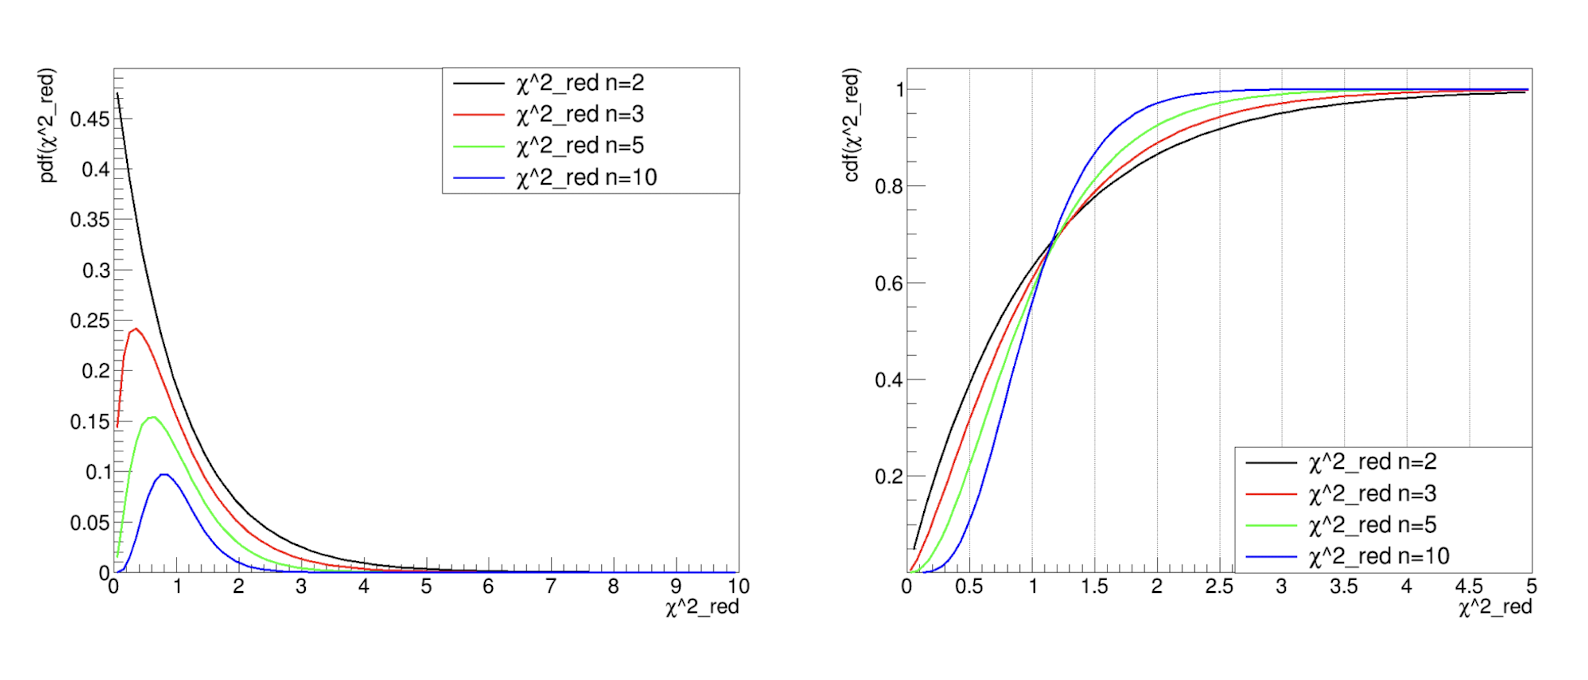
\includegraphics[scale = 0.5]{reducedChi}	
\centering
\vspace{0.in}
\caption{Distribuzione di $\chi^2$ ridotto e rispetti distribuzione cumulativa.}
\end{figure}
\end{document}
